% core-concepts.tex
% Section 2: What Should STILL Be Taught (Core Concepts)

%%%%%%%%%%%%%%%%%%%%
\section{What Should STILL Be Taught}
%%%%%%%%%%%%%%%%%%%%

%%%%%%%%%%%%%%%%%%%%
\begin{frame}{Core Concepts LLMs Cannot Replace}
  \begin{center}
    \textbf{Focus on concepts that require \underline{deep understanding}, not memorization.}
  \end{center}
  
  \vspace{0.3cm}
  
  \begin{enumerate}
    \item \textbf{Historical Development} --- Why languages evolved as they did
    \item \textbf{Design Philosophy} --- Minimalism (C) vs. Safety (Java)
    \item \textbf{Execution \& Memory Models} --- How programs actually run
    \item \textbf{Type Systems \& Runtime Systems} --- Static vs. dynamic guarantees
    \item \textbf{Interface/ABI Stability} --- Binary compatibility constraints
    \item \textbf{Cost Models} --- Compiler transformations, UB, virtual dispatch
  \end{enumerate}
  
  \vspace{0.3cm}
  
  \begin{alertblock}{Principle}
    Teach \textit{understanding} over \textit{recitation}. (cf. Perlis, Epigrams on Programming)
  \end{alertblock}
  
  % Speaker note: These are areas where human expertise provides irreplaceable value
\end{frame}
%%%%%%%%%%%%%%%%%%%%

%%%%%%%%%%%%%%%%%%%%
\begin{frame}{Historical Development of C}
  \begin{columns}[T]
    \begin{column}{0.5\textwidth}
      \textbf{Timeline:}
      \begin{itemize}
        \item 1969--1973: C developed at Bell Labs
        \item 1978: K\&R ``The C Programming Language''
        \item 1989: ANSI C (C89)
        \item 1999: C99 (VLAs, \texttt{restrict}, inline)
        \item 2011: C11 (atomics, threads)
        \item 2023: C23 (modern features)
      \end{itemize}
    \end{column}
    \begin{column}{0.48\textwidth}
      \textbf{Design Philosophy:}
      \begin{quote}
        ``Trust the programmer.'' \\
        ``Keep the language small and simple.'' \\
        ``Make it fast, even if not guaranteed portable.''
      \end{quote}
      \hfill --- \textit{Dennis Ritchie}
    \end{column}
  \end{columns}
  
  \vspace{0.3cm}
  
  \begin{block}{Teaching Point}
    Understanding \textit{why} C was designed this way explains undefined behavior, pointer arithmetic, and the lack of bounds checking.
  \end{block}
  
  % Speaker note: Reference "The Development of the C Language" (Ritchie, 1993)
\end{frame}
%%%%%%%%%%%%%%%%%%%%

%%%%%%%%%%%%%%%%%%%%
\begin{frame}[fragile]{Example 1: Pointer Aliasing and Undefined Behavior}
  \begin{columns}[T]
    \begin{column}{0.48\textwidth}
      \textbf{Strict Aliasing Rule:}
      \begin{block}{UB Example}
\begin{verbatim}
float f = 3.14f;
int *ip = (int *)&f;
int i = *ip;  // UB!
\end{verbatim}
      \end{block}
      
      \begin{block}{Correct Approach}
\begin{verbatim}
float f = 3.14f;
int i;
memcpy(&i, &f, sizeof(i));
\end{verbatim}
      \end{block}
    \end{column}
    \begin{column}{0.48\textwidth}
      \textbf{Why UB Exists:}
      \begin{block}{Signed Overflow}
\begin{verbatim}
int x = INT_MAX;
x = x + 1;  // UB!
\end{verbatim}
      \end{block}
      
      \textbf{Enables:}
      \begin{itemize}
        \item Loop optimizations
        \item Vectorization
        \item Dead code elimination
      \end{itemize}
    \end{column}
  \end{columns}
  
  \vspace{0.2cm}
  
  \begin{alertblock}{C99 Rationale}
    ``Undefined behavior gives the implementor license not to catch certain program errors...''
  \end{alertblock}
  
  % Speaker note: UB is a feature, not a bug---but must be taught carefully
\end{frame}
%%%%%%%%%%%%%%%%%%%%

%%%%%%%%%%%%%%%%%%%%
\begin{frame}[fragile]{Example 2: Memory Layout and Alignment}
  \begin{columns}[T]
    \begin{column}{0.48\textwidth}
      \begin{block}{Struct Definition}
\begin{verbatim}
struct example {
    char a;    // 1 byte
    int  b;    // 4 bytes
    char c;    // 1 byte
};
// sizeof = 12, not 6!
\end{verbatim}
      \end{block}
      
      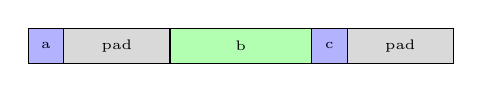
\begin{tikzpicture}[scale=0.45]
        \draw[fill=blue!30] (0,0) rectangle (1,1);
        \node at (0.5,0.5) {\tiny a};
        \draw[fill=gray!30] (1,0) rectangle (4,1);
        \node at (2.5,0.5) {\tiny pad};
        \draw[fill=green!30] (4,0) rectangle (8,1);
        \node at (6,0.5) {\tiny b};
        \draw[fill=blue!30] (8,0) rectangle (9,1);
        \node at (8.5,0.5) {\tiny c};
        \draw[fill=gray!30] (9,0) rectangle (12,1);
        \node at (10.5,0.5) {\tiny pad};
      \end{tikzpicture}
    \end{column}
    \begin{column}{0.48\textwidth}
      \begin{block}{Pointers to Pointers}
\begin{verbatim}
int x = 42;
int *p = &x;
int **pp = &p;
**pp = 100;  // x = 100
\end{verbatim}
      \end{block}
      
      \textbf{Real-World Uses:}
      \begin{itemize}
        \item Dynamic 2D arrays
        \item Linked list insertion
        \item Output parameters
      \end{itemize}
    \end{column}
  \end{columns}
  
  % Speaker note: Real-world impact on network protocols, file formats
\end{frame}
%%%%%%%%%%%%%%%%%%%%

%%%%%%%%%%%%%%%%%%%%
\begin{frame}[fragile]{Example 3: Library Design and Security}
  \textbf{P.J. Plauger's Principles + CERT C Secure Coding}
  
  \begin{columns}[T]
    \begin{column}{0.48\textwidth}
      \begin{block}{\texttt{gets} vs. \texttt{fgets}}
\begin{verbatim}
// DANGEROUS (removed in C11)
gets(buf);

// SAFE
fgets(buf, sizeof(buf), 
      stdin);
\end{verbatim}
      \end{block}
    \end{column}
    \begin{column}{0.48\textwidth}
      \begin{block}{STR31-C: Null termination}
\begin{verbatim}
strncpy(dest, src, 
        sizeof(dest));
dest[sizeof(dest)-1] = '\0';
\end{verbatim}
      \end{block}
    \end{column}
  \end{columns}
  
  \vspace{0.3cm}
  
  \textbf{Design Principles (Plauger):}
  \begin{itemize}
    \item Minimal interface, maximum functionality
    \item Composable primitives (\texttt{fopen}, \texttt{fread}, \texttt{fclose})
    \item Error handling via return values (not exceptions)
  \end{itemize}
  
  \textbf{Teaching Point:} Security vulnerabilities stem from misunderstanding semantics.
  
  % Speaker note: Reference SEI CERT C Coding Standard (2016)
\end{frame}
%%%%%%%%%%%%%%%%%%%%

%%%%%%%%%%%%%%%%%%%%
\begin{frame}[fragile]{Java Examples: Lambdas and GC Trade-offs}
  \begin{columns}[T]
    \begin{column}{0.48\textwidth}
      \textbf{Lambda Implementation:}
      \begin{block}{Source}
\begin{verbatim}
names.forEach(s -> 
    System.out.println(s));
\end{verbatim}
      \end{block}
      
      \textbf{Under the Hood:}
      \begin{itemize}
        \item \texttt{invokedynamic} instruction
        \item \texttt{LambdaMetafactory} generates class
        \item Captured vars become fields
        \item Explains ``effectively final''
      \end{itemize}
    \end{column}
    \begin{column}{0.48\textwidth}
      \textbf{GC vs. Manual Memory:}
      
      \textbf{\teal{Java GC:}}
      \begin{itemize}
        \item No use-after-free/double-free
        \item Simpler programming model
      \end{itemize}
      
      \textbf{\red{Java GC Costs:}}
      \begin{itemize}
        \item Stop-the-world pauses
        \item Memory overhead
        \item Unpredictable latency
      \end{itemize}
    \end{column}
  \end{columns}
  
  \vspace{0.2cm}
  
  \textbf{Teaching Point:} Students must understand \textit{why} both approaches exist.
  
  % Speaker note: Compare with C's malloc/free and C++'s RAII
\end{frame}
%%%%%%%%%%%%%%%%%%%%
